\scanpage{52}
\uline{\deleted{\unsure{Prop\textsuperscript{n}}}\unsure{Thme|Prop\textsuperscript{n}|Prop}} Le groupe $\operatorname{Aut}(C)$ est simplement transitif sur $\deleted{\unsure{\operatorname{Drap}}}\unsure{\operatorname{Rep}|\operatorname{Drap}}(C)$ (qui est \unsure{donc} un torseur \inserted{à g} sur $\operatorname{Aut}(C)$)

(On dit que $C$ est un pol (conv) \uline{régulier} quand il \deleted{\unsure{on}} \deleted{$\operatorname{Card}(\operatorname{Drap}(C))=2^n\cdot 2^{\unsure{n-1}}$} en est ainsi\ldots)

Le nb de facettes de dim $d+1$ contenant une facette donnée de dim $d$ est \deleted{$\unsure{2^d|2d}$} $(n-d)$, donc le nb des \deleted{drapeaux} \inserted{\unsure{rep.|drap.}} est
\[
2^n\cdot n\cdotn-1\cdot\ldots\,2\cdot1=2^n n!
\]
qui est aussi l'ordre de $\operatorname{Aut}(C)$. Il suffit de prouver que $\operatorname{Aut}(C)$ opère librement sur $\operatorname{Drap}(C)$, or c'est vrai pour tt polyèdre convexe :

\uline{Lemme} Soit $C$ un polyèdre convexe, $u$ un autom de $C$ fixant un drapeau de $C$. Alors $u$ est l'identité.

Récurrence sur $\dim C$. Pour $\dim C=0$, c'est triv. Soit $D=(F_0,\ldots,F_{n-1},F_n=C)$ le drapeau fixé. Par hyp. de récurrence, $u$ est l'identité sur $F_{n-1}$, car il fixe son \deleted{drapeau} \inserted{\unsure{rep.|drap.}} $(F_0,\ldots,F_{n-2},F_{n-1})$. Donc on a un autom \deleted{qui est} affine de $E_C=E$ qui \deleted{\unsure{f}}est l'identité sur un hyperplan $H=E_{F_{n-1}}$, et qui est d'ordre fini -- on voit facilement que c'est ou bien l'identité, ou bien une ``symétrie'' -- mais alors elle échange les deux $\frac12$ espaces déterminés par $H$, donc elle ne pourrait conserver $C$, OK.

\figure{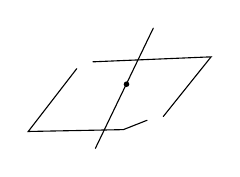
\begin{tikzpicture}[x=0.79cm,y=0.79cm,line cap=round]
\draw (0.78,1.01)--(0,0)--(1.53,0.03)--(1.91,0.18);
\draw (1.04,1.12)--(2.94,1.2)--(2.17,0.24);
\draw (1.08,-0.27)--(2.01,1.66);
\fill (1.58,0.76) circle (0.045);
\end{tikzpicture}}

\uline{Corollaire} Soit $C_0$ un cube de dim $n$, $D_0$ un drapeau du dit, \deleted{Al} $C$ un cube de dim $n$ Alors
\[
u\longmapsto u(D_0)\qquad\operatorname{Isom}(C_0,\deleted{\unsure{E}}C)\xrightarrow{\sim}\operatorname{Drap}(C)
\]
% archive sheet number: 51
